\documentclass{article}

\usepackage{graphicx}
\usepackage{tikz}
\usepackage{tikzsymbols}
\usetikzlibrary{calc,patterns,shapes.geometric}
\pagestyle{empty}
\usepackage[margin=0pt]{geometry}
\geometry{papersize={14in,12in}}

\def\centerarc[#1](#2)(#3:#4:#5){\draw[#1] ($(#2)+({#5*cos(#3)},{#5*sin(#3)})$) arc (#3:#4:#5);}

\begin{document}
	\begin{figure}
		\centering
		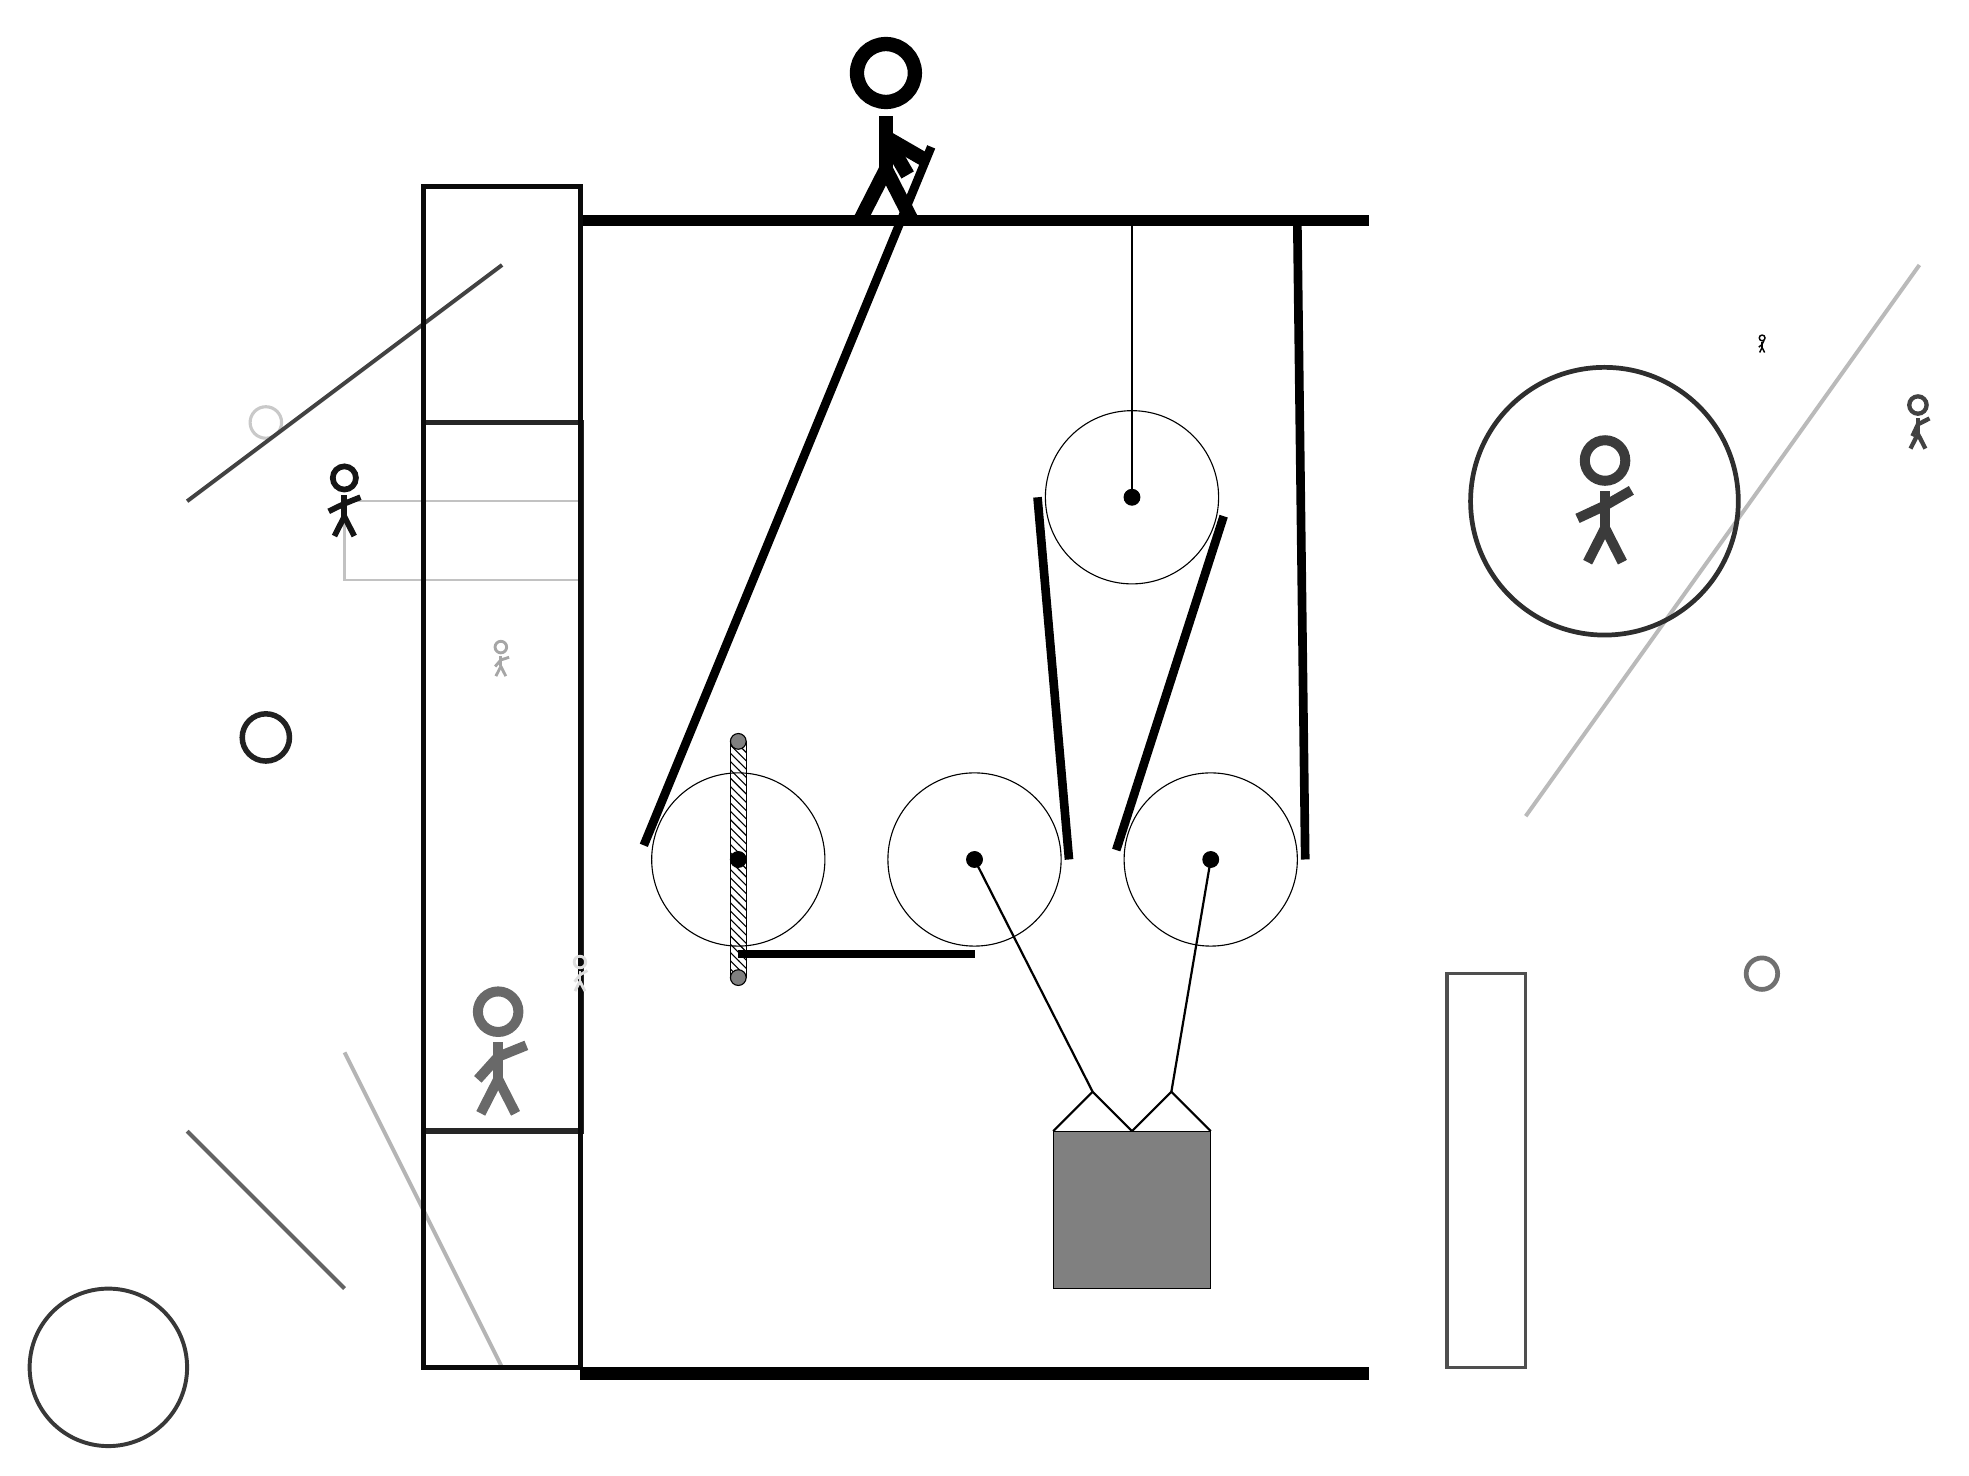
\begin{tikzpicture}
			%%%%% START %%%%%
			
			\draw[fill=black] (-4, 11.5) rectangle (6, 11.625);
			
			\draw (1, 3.45) circle (1.1);
			\draw[fill=black] (1, 3.45) circle (0.1);
			
			\draw (3, 8.05) circle (1.1);
			\draw[fill=black] (3, 8.05) circle (0.1);
			\draw[thick] (3, 8.05) -- (3, 11.5);
			
			\draw (4, 3.45) circle (1.1);
			\draw[fill=black] (4, 3.45) circle (0.1);
			
			\draw[thick] (4, 3.45) -- (3.5, 0.5);
			\draw[thick] (1, 3.45) -- (2.5, 0.5);
			\draw[thick]  (2, 0) -- (2.5, 0.5) -- (3, 0);
			\draw[thick]  (3, 0) -- (3.5, 0.5) -- (4, 0);
			\draw[fill=black!50] (2, 0) rectangle (4, -2);
			
			\draw (-2, 3.45) circle (1.1);
			\draw[fill=black] (-2, 3.45) circle (0.1);
			\draw[pattern=north west lines, pattern color=black] (-2.1, 4.95) rectangle (-1.9, 1.95);
			\draw[fill=black!50] (-2, 4.95) circle (0.1);
			\draw[fill=black!50] (-2, 1.95) circle (0.1);
			
			\draw[line width=1.1mm] (0.45, 12.5) -- (-3.2, 3.63);
			\centerarc[line width=1.1mm](-2, 3.45)(160:270:1.2000000000000002);
			\draw[line width=1.1mm](-2, 2.25) -- (1, 2.25);
			\centerarc[line width=1.1mm](1, 3.45)(270:360:1.2000000000000002);
			\draw[line width=1.1mm] (2.2, 3.45) -- (1.8, 8.05);
			\centerarc[line width=1.1mm](3, 8.05)(-20:180:1.2000000000000002);
			\draw[line width=1.1mm](4.164, 7.81) -- (2.8, 3.57);
			\centerarc[line width=1.1mm](4, 3.45)(160:360:1.2000000000000002);
			\draw[line width=1.1mm](5.2, 3.45) -- (5.1, 11.5);
			
			\node at (-0.07, 12.7) {\Strichmaxerl[10][120][-30]};
			
			\node[line width=0.4mm, color=black!59] at (-5, 1) {\Strichmaxerl[7][48][22]};
			
			\draw [line width=0.4mm, color=black!21](-8, 9) circle (0.2);
			\draw [line width=0.5mm, color=black!78](-10, -3) circle (1.0);
			\draw[line width=0.5mm, color=black!61](-7, -2) -- (-9, 0);
			\draw[line width=0.5mm, color=black!29](-7, 1) -- (-5, -3);
			
			\draw[line width=0.5mm, color=black!27](8, 4) -- (13, 11);
			\draw [line width=0.6mm, color=black!82](9, 8) circle (1.7);
			
			\draw[line width=0.5mm, color=black!34] (-6, -1) rectangle (-6, 12);
			\draw[line width=0.7mm, color=black!85] (-6, 9) rectangle (-4, 0);
			\draw[line width=0.3mm, color=black!24] (-4, 8) rectangle (-7, 7);
			
			\draw[line width=0.5mm, color=black!74](-5, 11) -- (-9, 8);
			\draw [line width=0.6mm, color=black!56](11, 2) circle (0.2);
			\draw[line width=0.6mm, color=black!96] (-6, -3) rectangle (-4, 12);
			\node[line width=0.7mm, color=black!74] at (13, 9) {\Strichmaxerl[3][65][27]};
			\draw[line width=0.4mm, color=black!69] (7, 2) rectangle (8, -3);
			\node[line width=0.3mm, color=black!77] at (9, 8) {\Strichmaxerl[7][25][30]};
			\node[line width=0.6mm, color=black!99] at (11, 10) {\Strichmaxerl[1][40][64]};
			\draw [line width=0.7mm, color=black!87](-8, 5) circle (0.3);
			\node[line width=0.5mm, color=black!13] at (-4, 2) {\Strichmaxerl[2][52][30]};
			\node[line width=0.2mm, color=black!92] at (-7, 8) {\Strichmaxerl[4][26][22]};
			\node[line width=0.6mm, color=black!35] at (-5, 6) {\Strichmaxerl[2][49][18]};
			
			\draw[fill=black] (-4, -3) rectangle (6, -3.15);
			
			%%%%% END %%%%%
		\end{tikzpicture}
	\end{figure}	
\end{document}